\documentclass[11pt]{article}
\usepackage{amsmath}
\usepackage[utf8]{inputenc}

\usepackage{xcolor}
\usepackage{setspace}
\usepackage{graphicx}
\usepackage[hidelinks,colorlinks=true,linkcolor=blue,citecolor=blue]{hyperref}

\newcommand{\blue}[1]{\textcolor{blue}{#1}}
\newcommand{\red}[1]{\textcolor{red}{#1}}
\newcommand{\link}[1]{\href{#1}{\blue{#1}}}

\definecolor{keywordred}{RGB}{255, 123, 114}
\definecolor{keywordorange}{RGB}{255, 166, 86}
\definecolor{keywordpurple}{RGB}{210, 168, 254}
\definecolor{commentblue}{RGB}{165, 214, 255}
\definecolor{noneblue}{RGB}{121, 192, 255}

\title{Recursive Algorithms for Parsing the Ram Scripting Language into Abstract Syntax Trees in Python}
\author{William S. Assad\footnote{Department of Mathematics, University of Toronto} , Ariel Chouminov\footnote{Department of Computer Science, University of Toronto} , \\ Ramya Chawla$^\dag$, Zain Lakhani$^\dag$}
\date{April 16, 2021}

\begin{document}

\maketitle

\begin{abstract}
    For the student of Computer Science, we introduce a systematic algorithm for parsing a new scripting language into Abstract Syntax Trees (ASTs) in Python. An induction-based structure for parsing is used where the base case represents an instance of \texttt{Line} and the recursive step represents an instance of a \texttt{Block} child (enumerated type). Once the nested structure is created, we recursively parse each object into a specific AST. The conventional approach is used for the evaluate method; the abstract classes \texttt{Statement} and \texttt{Expr} are defined. Instead of presenting a standard technical parsing algorithm, \emph{Ram} is implemented with minimal emphasis on asymptotic running-time complexity. Like Python, many features of \emph{Ram} are ``syntactic sugar''. We see that for an input family of $n$ lines of \emph{Ram} code and maximum nesting of depth $k$, the average running time complexity of the \texttt{.parse} and \texttt{.evaluate} algorithm is $\mathcal{O}(kn)$.
\end{abstract}

\section{Introduction and Theory}
Programming languages are built using Abstract Syntax Trees (ASTs), a recursive data structure that represents written code \cite{david}. Programmers write code in the form of large strings, which are parsed into ASTs and recursively evaluated \cite{david, ASTs}. As humans, we often take this necessary translation for granted, given that we can simply read programs as text \cite{david}. Any computer, however, will interpret this text, translate it several times, and then produce an output with incredible efficiency. 

Programming languages present humans the opportunity to interact with computers in unique ways. One of these languages is \href{https://www.python.org/}{Python}, a high-level programming language that is relatively easy to learn. While it has many advantages as a first programming language for new programmers, there are some key disadvantages. Mainly, it differs structurally from other programming languages in terms of indented blocks and variables that represent multiple data types\footnote{Indentation in Python represents nesting instead of standard curly braces.}. This means it offers beginner programmers an introduction into the world of programming while making their transition into other languages quite difficult. 

Translation to English is another key obstacle in introducing programming languages to new students of Computer Science. The intuition behind writing certain lines of code is often masked by the nuances of a particular language. For example, there is no obvious reason why the line of Python code \texttt{print([(x, x \% 2 == 0) for x in range(10)])} should display a list of numbers from 0 to 9 and whether or not they are even. Hence, {we introduce the programming language (Ram) to be easily translatable to English and help better prepare beginner programmers to use other languages.} We discuss a method of implementing the \emph{Ram} programming language in Python using a systematic algorithm.

\section{Implementation}

\subsection{Ram Syntax}

Before diving directly into the code and our plan of implementation, we will clearly define all the syntactical structure of \emph{Ram} code. We emphasize the readability of this code and the fluency with which it can be translated to English. \hyperlink{tab1}{Table 1} and \hyperlink{tab2}{Table 2} contain various statements in Python with a side-by-side comparison of their equivalent statements in \emph{Ram}.

\begin{center}
    \begin{spacing}{1.1}
    
        \hypertarget{tab1}{}
    
        \begin{tabular}{|l|l|} 
             \hline
             
             \textbf{Python Syntax} & \textbf{Ram Syntax} \\ 
             
             \hline
             \texttt{for x in \red{range(5)}:} & \texttt{loop with x \red{from 0 to 4} \{ } \\ 
             \quad \quad \texttt{print(x)} & \quad \quad  \texttt{display x} \\
              & \} \\
             
             \hline
             
             \texttt{\red{x} = 5} & \texttt{\red{set integer} x to 5} \\
             
             \hline
             
             \texttt{\red{letters} = `hello'} & \texttt{\red{set text} letters to ``hello''} \\
             
             \hline
             
        \end{tabular}
        
        $ $
        
        \small{\hyperlink{tab1}{Table 1}: Comparison of Python and Ram Syntax}
             
        \begin{tabular}{|l|l|} 
             \hline \hypertarget{tab2}{}
             
             \textbf{Python Syntax} & \textbf{Ram Syntax} \\ 
             
             \hline
             
             % \texttt{\red{def} f(x:\,int) -> None:} & \texttt{\red{new function} f takes (x) \{ } \\
             % \quad \quad \texttt{x = x - 5} & \quad \quad \texttt{\red{reset x} to x - 5} \\
             % \quad \quad \texttt{print(x)} & \quad \quad \texttt{display x} \\
             %  & \} \\
              
             % \hline
             
             \texttt{\red{var1} = 10} & \texttt{\red{set integer} var1 to 10} \\
             
             % \quad \quad & \quad \quad \\
             
             \texttt{\red{if} var1 \red{==} f(8):} & \texttt{\red{if} var1 \red{is} f[x=8] \{ } \\
             
             \quad \quad \texttt{print(`Equal!')} & \quad \quad \texttt{display ``Equal!''} \\
             
             \texttt{\red{elif} (var1 + var2) \red{==} 5:} & \texttt{\} \red{else if} (var1 + var2) \red{is} (5) \{ } \\
             
             \quad \quad \texttt{print(`Equals 5')} & \quad \quad \texttt{display ``Equals 5''} \\
             
             \texttt{\red{else}: } & \texttt{\} \red{else} \{} \\
             
             \quad \quad \texttt{print(`:(')} & \quad \quad \texttt{display ``:(''} \\
              
             \quad \quad & \texttt{\}} \\
             
             \hline 
             
             \texttt{\red{def} f(x, y) -> int:} & \texttt{\red{new function} f takes (x,y) \{ } \\
             \quad \quad \texttt{x = x + y} & \quad \quad \texttt{\red{reset integer x} to x + y} \\
             \quad \quad \texttt{\red{return} x} & \quad \quad \texttt{\red{send back} x} \\
              & \} \\
              
             \hline
        \end{tabular}
    
    \end{spacing}
    
    \bigskip
    
    \small{\hyperlink{tab2}{Table 2}: Comparison of Python and Ram Syntax}
    
\end{center}

\subsection{AST Implementation}

Processing \emph{Ram} code ultimately results in the creation of ASTs, which we define in Python. We begin by defining various statements and expressions including (but not limited to) for-loops, functions, if-statements, assignment statements, and print statements. Class inheritance is structured using an abstract class representing a statement, \texttt{Statement}, and an abstract subclass representing an expression, \texttt{Expr} (\hyperlink{fig1}{Figure 1}).

\bigskip

\hypertarget{fig1}{}

\texttt{\textcolor{keywordred}{class} \textcolor{keywordorange}{Statement}:}

\quad\quad \texttt{\textcolor{commentblue}{"""An abstract class representing a Python statement.}}

\quad\quad{\texttt{\textcolor{commentblue}{"""}}}

\quad\quad\texttt{\textcolor{keywordred}{def} \textcolor{keywordpurple}{evaluate}(self,\,env:\,\textcolor{keywordorange}{dict[str, Any]}) -> Optional[Any]:}

\quad\quad\texttt{"""Evaluate the statement in a given environment."""}

\quad\quad \quad\quad \texttt{\textcolor{keywordred}{raise} \textcolor{keywordorange}{NotImplementedError}}

\bigskip

\texttt{\textcolor{keywordred}{class} \textcolor{keywordorange}{Expr}:}

\quad\quad \texttt{\textcolor{commentblue}{"""An abstract class representing a Python expression.}}

\quad\quad{\texttt{\textcolor{commentblue}{"""}}}

\quad\quad\texttt{\textcolor{keywordred}{def} \textcolor{keywordpurple}{evaluate}(self,\,env:\,\textcolor{keywordorange}{dict[str, Any]}) -> Optional[Any]:}

\quad\quad\texttt{"""Evaluate the statement in a given environment."""}

\quad\quad \quad\quad \texttt{\textcolor{keywordred}{raise} \textcolor{keywordorange}{NotImplementedError}}

\bigskip

\begin{center}
    \small{\hyperlink{fig1}{Figure 1}: \texttt{Statement} and \texttt{Expr} Abstract Classes}
\end{center}

ASTs are a form of trees since a \texttt{Statement} can be composed of many \texttt{Expr}'s which can also be composed of many different other \texttt{Expr}'s, which represent subtrees. For example, a binary operation expression \texttt{BinOp(Expr)} is defined in terms of a left \texttt{Expr} and a right \texttt{Expr} as seen in \hyperlink{fig2}{Figure 2}. This allows for any form of nesting, provided that the left and right subtrees evaluate to  floating-point values (leafs are instances of \texttt{Num} or \texttt{Name}). All other ASTs have a similar structure, being composed of other statements and expressions.

\begin{center}
    \hypertarget{fig2}{}

    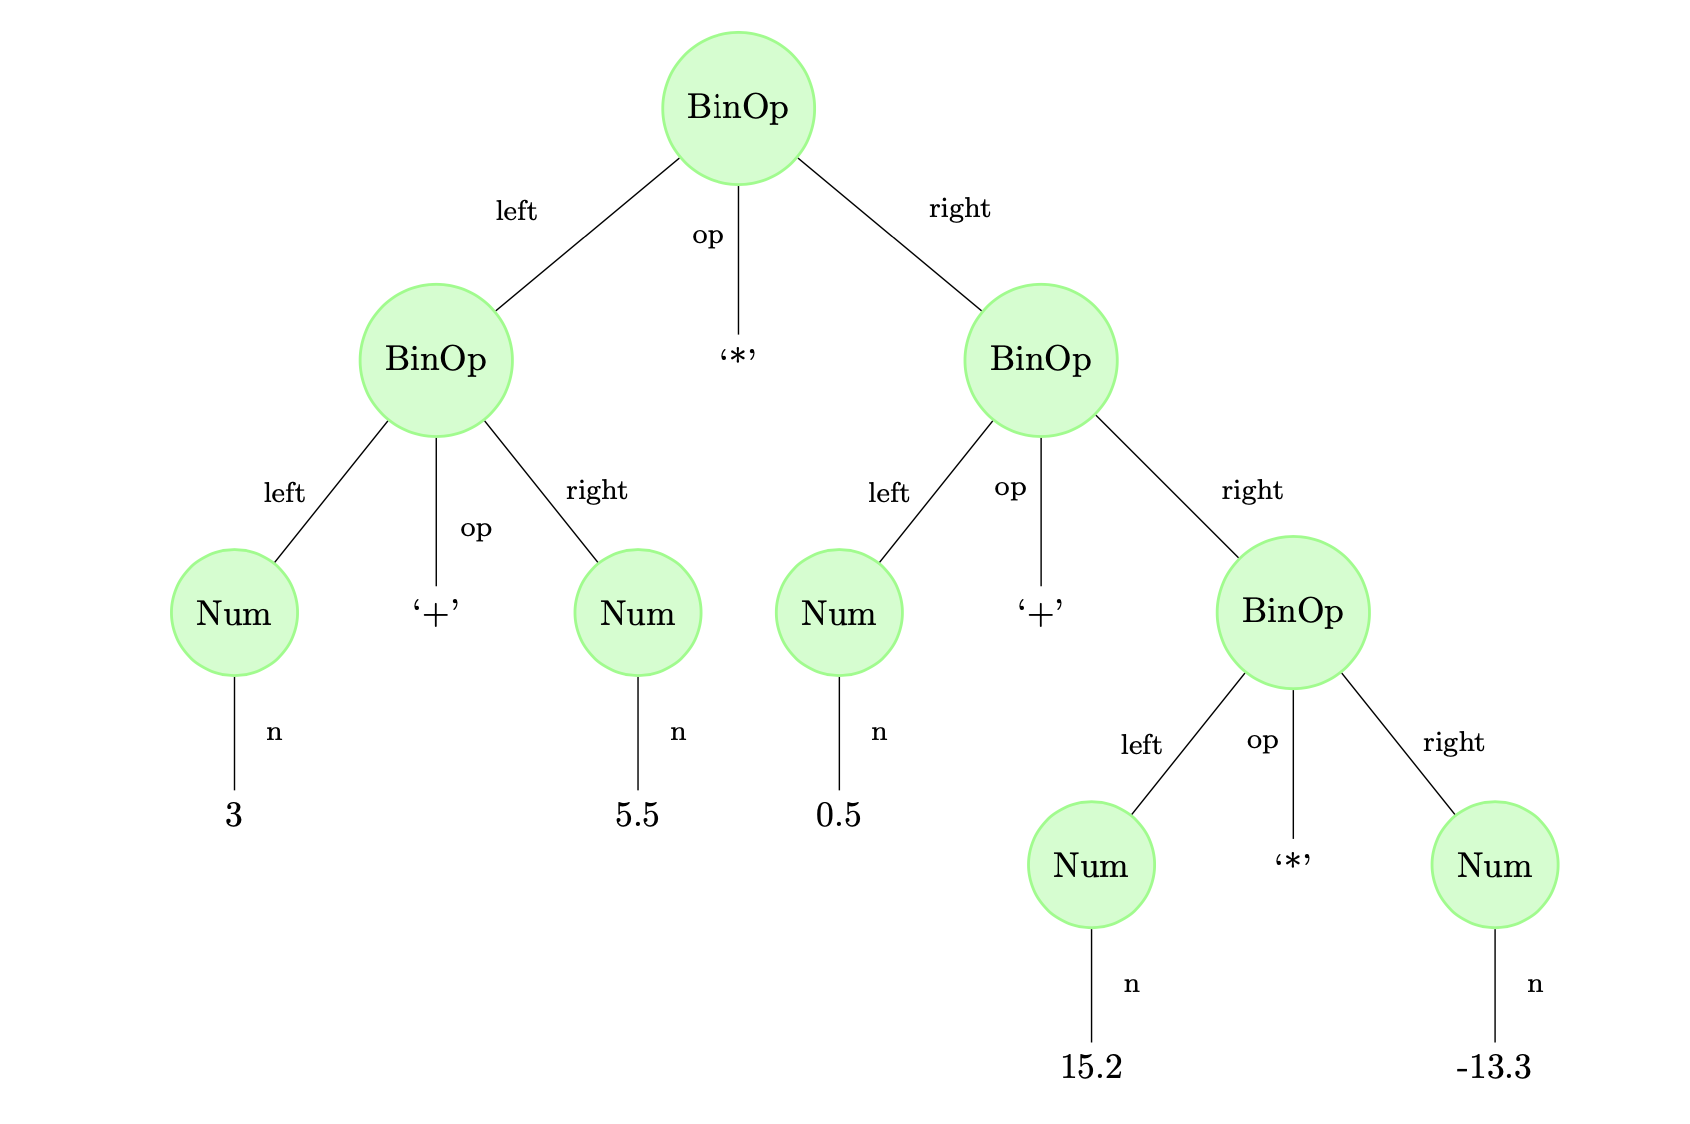
\includegraphics[scale=0.4]{binop2.png}
    
    \small{\hyperlink{fig2}{Figure 2}: \texttt{BinOp} Tree Structure \cite{david}}
    
    $ $
\end{center}

\subsection{Parsing Algorithms}

Instead of reading from left to right, the interpreter must convert linear plain text into the deeply nested AST structures seen in \hyperlink{fig2}{Figure 2}. This is the process of parsing. More formally, parsing is the process of analyzing a string of symbols and or words that are presented in either natural language, computer language, or data structure and converting them into ASTs \cite{def}. Like Python, the code written by our users will initially be processed as the basic data types --- strings, booleans, and integers. For example, the ram data type \texttt{text} is equivalent to the AST \texttt{String} whose \texttt{evaluate} method returns a Python \texttt{str}. Here we describe in detail the four step parse and evaluate algorithm.

\begin{enumerate}
    \item \textcolor{red}{Read in the \texttt{.ram} file as a list of tuples.}
    
    The \texttt{.ram} file is read in as a list of tuples where each tuple contains the line and the line number. 
    
    \item \textcolor{red}{Recursively create the nested block structure.} \hypertarget{step2}{}
    
    In \texttt{parsing.py}, we introduce an abstract class \texttt{Block} (\hyperlink{fig3}{Figure 3}) which has three sub-classes --- \texttt{Loop}, \texttt{Function}, and \texttt{If}. A complicated recursive algorithm \texttt{make\_child} that runs in \texttt{Block.\_\_init\_\_} creates the proper nested structure. The function determines the block type of the caller and creates a new specific block instance. The newly created block recursively parses through all of its children, which runs through the same process as the parent. The parent class assigns its caller a new sub-class type (for example a \texttt{LoopBlock}), such that when the block is parsed, the parsing specific to that block type is executed. Similar to \texttt{Statement} and \texttt{Expr}, these classes and sub-classes are used to create a nested structure. The use of these classes allows us to recursively parse each block of code. 
    
    \item \textcolor{red}{Recursively parse the nested block structure.}
    
     Each type of \texttt{Line} and child of \texttt{Block} has its own \texttt{parse} method which recursively creates an AST. For example, \texttt{IfBlock.parse} would return the \texttt{If(Statement)} AST.
    
    \item \textcolor{red}{Evaluate the resulting ASTs.}
    
    As described in \hyperlink{fig1}{Figure 1}, each AST has an \texttt{evaluate} method. For example, \texttt{BinOp.evaluate} would return a floating point value, as represented in Python.
    
\end{enumerate}

\bigskip

\hypertarget{fig3}{}
    
\quad \texttt{\textcolor{keywordred}{class} \textcolor{keywordorange}{Block}:}
    
\quad \quad\quad \texttt{\textcolor{commentblue}{"""A block of Ram code to parse. """}}

\quad \quad\quad\texttt{\textcolor{keywordred}{def} \textcolor{keywordpurple}{parse}(self) -> Statement:}
    
\quad \quad\quad \texttt{\textcolor{commentblue}{"""Parse a block of Ram code."""}}
    
\quad \quad\quad \quad\quad \texttt{\textcolor{keywordred}{raise} \textcolor{keywordorange}{NotImplementedError}}

\bigskip

\begin{center}

    \small{\hyperlink{fig3}{Figure 3}: \texttt{Block} Abstract Class}
\end{center}

\newpage

\emph{Ram} is intended to support simple arithmetic expressions, including the use of brackets. Regardless of the number of smaller computations that are nested within any binary operation, we need to evaluate the expression in terms of the order of operations. We were able to successfully implement very complex recursive algorithms such as \texttt{lexify} and \texttt{pedmas} in \textit{parsing/parse\_numeric.py}. Recursion was an essential tool in many algorithms; without it, we would have great difficulty locating and keeping track of various blocks of code. To give an example of this process, let's run through the specific algorithm for parsing this line of Ram code:

\begin{center}
    \texttt{\red{set integer} var1 to 4 * 3 + (8 - 4 * 2)}
\end{center}

We first read the line as a tuple consisting of the line itself as a string and the corresponding line number in the enclosing file. The keyword \texttt{set} is detected, meaning the line is to be parsed as a variable assignment statement. The keyword \texttt{integer} is then detected, meaning the line is to be parsed more specifically as a numerical value. The variable name, \texttt{var1}, is stored and the numeric expression \texttt{4 * 3 + (8 - 4 * 2)} is run through the \texttt{lexify} algorithm. This algorithm is fairly complex, using recursion to create the relevant nesting structure around the binary operations, following the mathematical order of operations. Once this process is finished, \texttt{var1} is assigned to the \texttt{BinOp} AST returned by the \texttt{Line.parse} method. Finally, the statement is evaluated and the environment is updated to contain the new variable.

The intuition is to take blocks of code and separate them into loop blocks, if blocks, and function blocks. Then the body portion of those blocks can contain nested blocks within, and this forms the nested structure we addressed earlier. Once these blocks are parsed, the program is able to treat them as functions and can accurately identify and interpret each statement of code.

We also ensure that the nesting of the blocks occurs in the correct order through the \texttt{process\_ram} function in \texttt{process.py}. This function takes in \emph{Ram} code as a list of tuples in the form: $\texttt{[(<line>,}$ $\texttt{<line\_number>), \dots]}$ and returns a list which correctly nests the blocks provided. This transform the data into the proper nested structure that is assumed in step (\hyperlink{step2}{2}) of the parse and evaluate algorithm. This nested structure is directly associated with trees--- a non-binary tree where each node has one child and each child represents another layer of nesting.

As a result of the combination of these ASTs, we are able to successfully create an interactive component and allow the user to freely experiment with Ram code and even build simple programs.

Referencing external libraries, we used \texttt{sys}, \texttt{os} and \texttt{platform}, which all come packaged with python and do not require any additional installation. We used \texttt{sys} to read the command line argument when calling \texttt{ram <filepath>.ram} in order to get the file path in the \texttt{verify\_file} function in \texttt{process.py}. In \texttt{install.py}, \texttt{platform} and \texttt{os} are used in the \texttt{InstallRam} class. An alias that links to an executable \texttt{main.py} is created at \texttt{usr/local/bin/ram} using \texttt{os}. This is only done (using \texttt{platform}) provided the platform is Darwin.


\section{Discussion}

Upon testing numerous different sample files with many different variations of code --- a combination of assignment statements, loops, if statements, and functions all nested within one another --- the four step parse and evaluate algorithm accurately processes \emph{Ram} code.

We were able to successfully create a new programming language that is easily translatable to English and helps better prepare beginner programmers to use another programming language. The syntax that we had in mind was properly executed and properly reinforced; when users do not correctly follow the \emph{Ram} syntax requirements, the appropriate \texttt{RamException} is raised.

\section{Notes and Acknowledgement}

See the \href{https://github.com/willassad/ram}{GitHub} repository for instructions on how to install \emph{Ram} and write simple code in \texttt{.ram} files. All forms of distribution of the code, whether as given or with any changes,
are expressly prohibited. All files are Copyright \copyright \, 2021 Will Assad, Zain Lakhani, Ariel Chouminov, and Ramya Chawla.

\bigskip

\noindent The development of this project (motivation and theory) would not be possible without \emph{CSC111} and \href{https://www.cs.toronto.edu/~david/}{David Liu} at the University of Toronto.

\newpage

\begin{thebibliography}{9}

\bibitem{david}
David Liu. \textit{CSC111 Lectures}. University of Toronto. 2021.

\bibitem{ASTs}
Dennis Howe. \textit{Free On-line Dictionary of Computing}. Internet Encyclopedia Project. 2008.

\bibitem{pyAST}
\textit{Abstract Syntax Trees}. Python Documentation. Available from: \link{https://docs.python.org/3/library/ast.html}

\bibitem{pyNLTK}
\textit{Natural Language Toolkit}. Python Documentation. Available from: \link{https://www.nltk.org/}

\bibitem{def}
Chapman, Nigel P. \textit{LR Parsing: Theory and Practice, Cambridge University Press}. 1987.

\end{thebibliography}

\end{document}